\section*{AI/ML Solution Technical Overview}

\subsection*{Data Collection \& Preprocessing}

\subsubsection*{Data Sources}
Medical School Material Slides \\

\vspace{-14pt}
\begin{tabular}{ll}
Format and Size & : PDF and PPTX, 10 documents, each 22 to 122 pages/slides \\
Slide structure & :
\end{tabular}
\begin{itemize}[itemsep=0pt,topsep=0pt]
    \item Title \& subtitle
    \item Content
    \item Table
    \item Flowcharts
    \item Diagram with labels
    \item Other images
\end{itemize}

\subsubsection*{Data Cleaning}



\begin{itemize}
    \item{Format Standardization} \\
    Source materials are provided in both PDF and PPTX formats. To ensure consistent downstream processing, PPTX files are converted into PDF format using the LibreOffice CLI. This provides a uniform input format for the subsequent document processing pipeline.
    
    \item{saldkmasd}
    
\end{itemize}


Removing irrelevant data from the slides, such as:
\begin{itemize}[itemsep=0pt,topsep=0pt]
    \item header \& footer
    \item decorative image
\end{itemize}
\begin{figure}[htbp]        
    \centering
    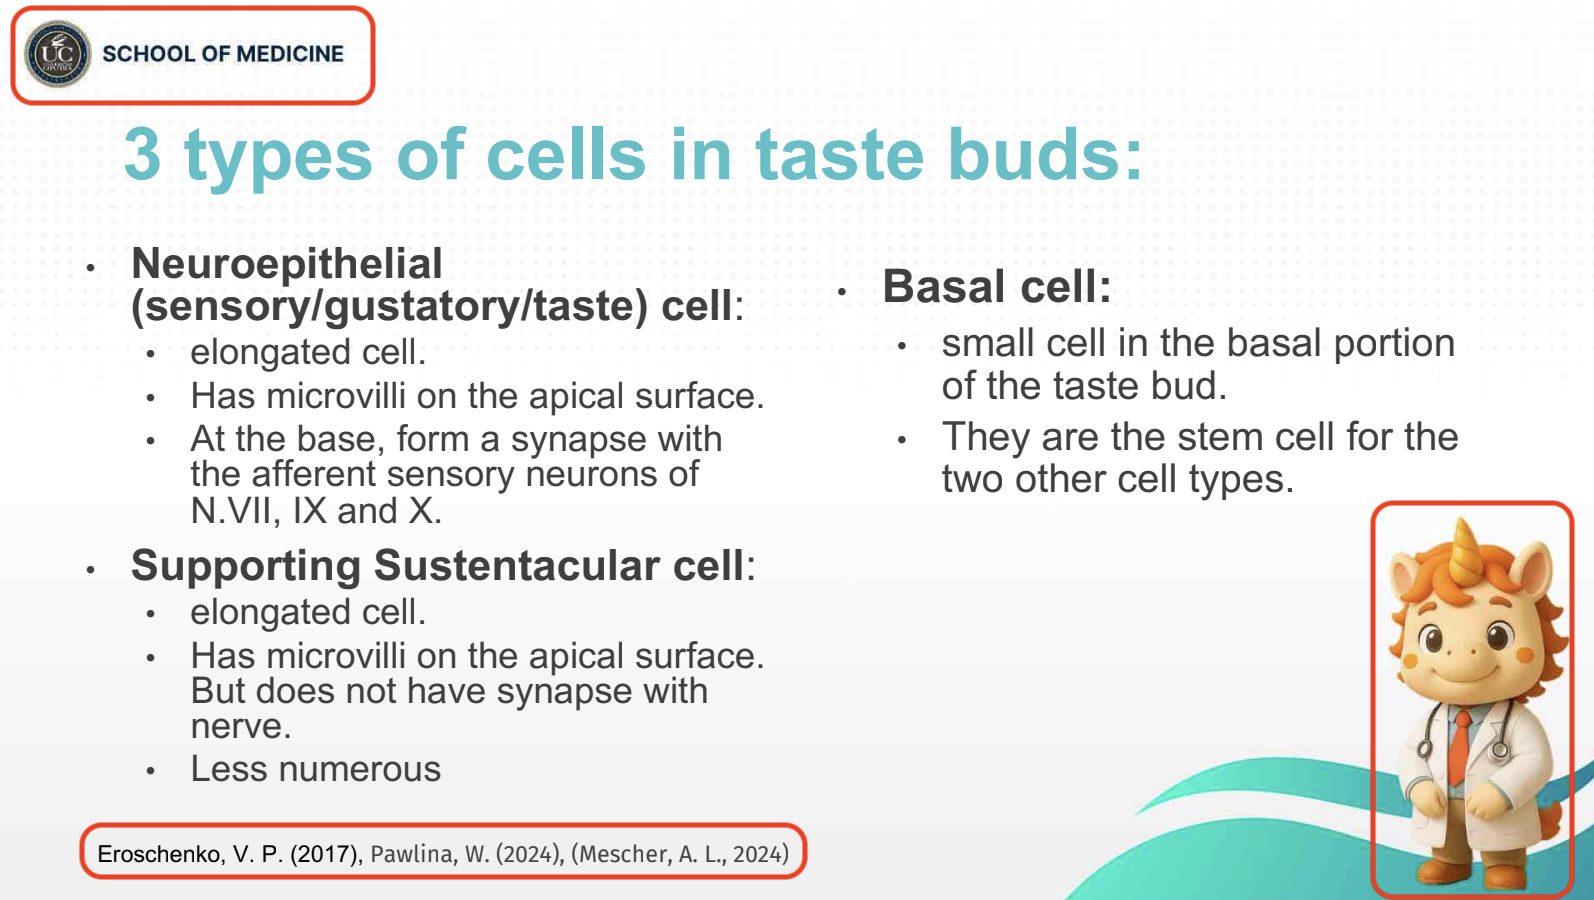
\includegraphics[width=0.45\textwidth]{images/noise1.png}
    \hfill
    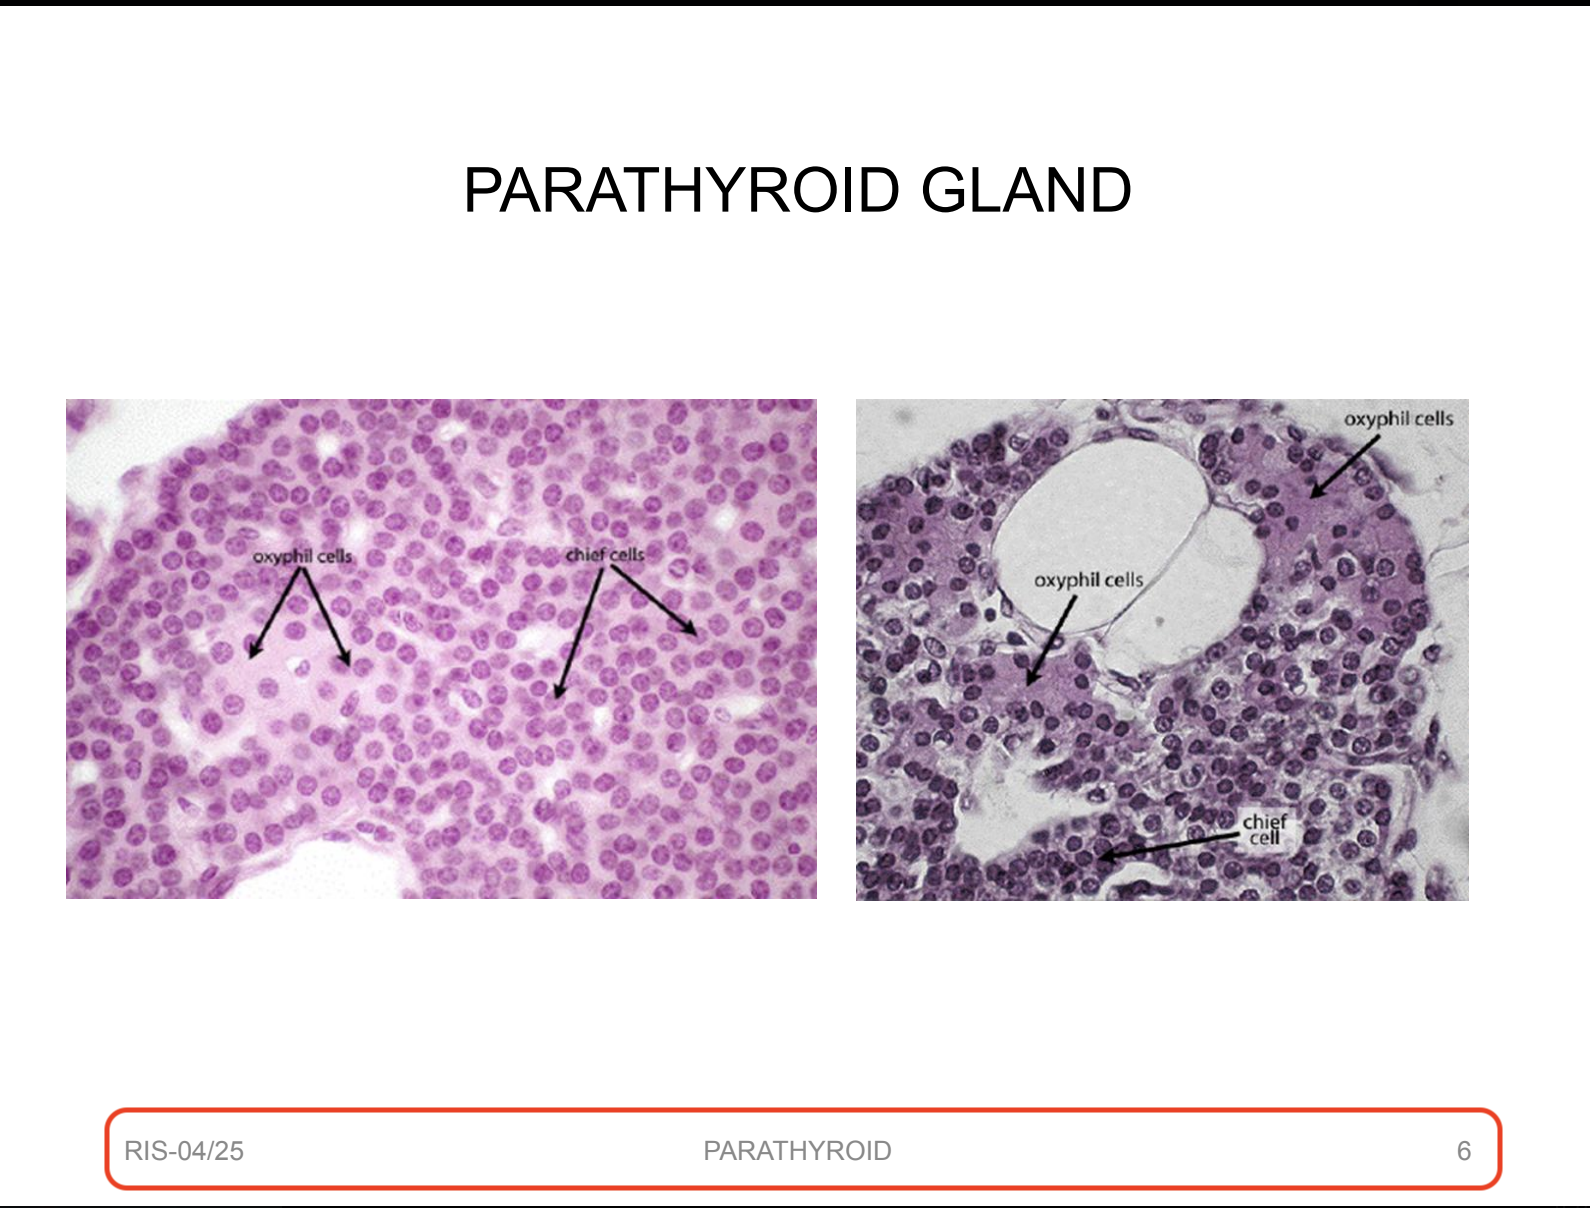
\includegraphics[width=0.45\textwidth]{images/noise2.png}
    % \caption{Two images side by side.}
    % \label{fig:two-images}
\end{figure}


\subsubsection*{Data Preprocessing}

\subsubsection*{Feature Engineering}

%%%%%%%%%%%%%%%%%%%%%%%%%%%%%%%%%%%%%%%%%%%%%%%
\subsection*{Exploratory Data Analysis}

Explain:
\begin{itemize}
    \item Key insights
    \item Visualization methods
    \item Statistical findings
\end{itemize}
%%%%%%%%%%%%%%%%%%%%%%%%%%%%%%%%%%%%%%%%%%%%%%%
\subsection*{Model Experiment}

Document your experiments systematically.

For each model, include:
\begin{itemize}
    \item Model architecture
    \item Why it was chosen
    \item Hyperparameters
    \item Training procedure
    \item Evaluation metrics
    \item Results
\end{itemize}

\subsection*{Conclusion}

Summarize:
\begin{itemize}
    \item Final model selected
    \item Why it performs best
    \item Comparison with other models
    \item Final performance metrics
\end{itemize}